% !Mode:: "TeX:UTF-8"
\chapter{实践:设计SLAM系统}
\begin{mdframed}  
	\textbf{主要目标}
	\begin{enumerate}[labelindent=0em,leftmargin=1.5em]
		\item 实际设计一个视觉里程计。
		\item 理解SLAM软件框架是如何搭建的。
		\item 理解在VO设计中容易出现的问题,以及修补的方式。
	\end{enumerate}
\end{mdframed}

本讲是全书的总结部分。我们将用到前面所学的知识,实际书写一个视觉里程计程序。你会管理局部的机器人轨迹与路标点,并体验一下一个软件框架是如何组成的。在操作过程中,我们会遇到许多实际问题:如何对图像进行连续的追踪,如何控制BA的规模,等等。为了让程序稳定运行,我们需要处理以上的种种情况,这将带来许多工程实现方面的、有益的讨论。

\newpage 
\section{为什么要单独列工程章节?}
知晓砖头和水泥的原理,并不代表能够建造伟大的宫殿。

在笔者深爱的《我的世界》游戏中,玩家拥有的只是一些色彩、纹理不同的方块。其性质极其简单,而玩家所要做的只是把这些方块放在空地上而已。理解一个方块至为简单,但实际拿起它们时,初学者往往只能搭建简单的火柴盒房屋,而有经验、有创造力的玩家则可用这些简单的方块建造民居、园林、楼台亭榭,乃至城市(\autoref{fig:mcarchitecture}~)\footnote{左下是我的练习作品。右下来自Epicwork团队作品:《圆明园》。我曾经在Epicwork中学习过一段时间,那里的年轻人甚至小朋友们的创造力给我留下了深刻的印象。}。

\begin{figure}[!htp]
	\centering    
	\includegraphics[width=0.9\linewidth]{designVO/mcarchitecture}\\
	\caption{从简单的事物出发,逐渐搭建越来越复杂但越来越优秀的作品。}
	\label{fig:mcarchitecture}
\end{figure}

在SLAM中,我们认为工程实现和理解算法原理应该至少是同等重要的,甚至更应强调如何书写实际可用的程序。算法的原理,就像一个个方块一样,我们可以清楚明确地讨论它们的原理和性质,但仅仅理解了一个个方块并不能使你建造真正的建筑:它们需要大量的尝试、时间和经验,我们鼓励读者朝更为实际的方向努力——当然这往往是十分复杂的。就像在《我的世界》里那样,你需要掌握各种立柱、墙面、屋顶的结构,墙面的雕花,几何形体角度的计算,这些远远不像讨论每个方块的性质那样简单。

SLAM的具体实现亦是如此,一个实用的程序会有很多的工程设计和技巧(Trick),还需要讨论每一步出现问题之后该如何处理。原则上讲,每个人实现的SLAM都会有所不同,多数时候我们并不能说哪种实现方式就一定是最好的。但是,我们通常会遇到一些共同的问题:“怎么管理地图点”“如何处理误匹配”“如何选择关键帧”,等等。我们希望读者能对这些可能出现的问题产生一些直观的感觉——我们认为这种感觉是非常重要的。

\clearpage
所以,出于对实践的重视,本讲我们将带领读者领略一下搭建SLAM框架的过程。就像建筑那样,我们要讨论柱间距、门面宽高比等琐碎但重要的问题。SLAM工程是复杂的。即使我们只保留核心的部分,也会占用大量的篇幅,使本书变得过于繁冗。不过,请注意,尽管完成之后的工程是复杂的,但是中间的“由简到繁”的过程,是值得详细讨论、有学习价值的。所以,我们要从简单的数据结构出发,先来做一个简单的视觉里程计,再慢慢地把一些额外的功能加进来。换言之,我们要把\textbf{从简单到复杂}的过程展现给读者看,这样你才会明白一个库是如何像雪人那样慢慢堆起来的。

本讲的代码放在slambook2/ch13中。我们将实现一个精简版的双目VO,然后看看它在Kitti数据集中的运行效果。这个VO由一个光流追踪的前端和一个局部BA的后端组成。为什么要选双目VO呢?其一是双目实现相对简单,只需单帧即可完成初始化;其二是双目存在3D观测,实现效果也会比单目较好。

\section{工程框架}
我们讨论的是一个工程实现,而工程通常是有一个框架的概念。大多数Linux库都会按照模块对算法代码文件进行分类存放,譬如头文件会放在头文件目录中,源代码则放在源代码目录中。此外,可能还有配置文件、测试文件、三方库等等。现在我们来按照小型算法库的普遍做法来分类我们的文件:

\begin{enumerate}
    \item 在bin下存储编译好的二进制文件;
	\item include/myslam	存放SLAM模块的头文件,主要是.h文件。这种做法的理由是,当把包含目录设到include,引用自己的头文件时,需要写include \texttt{"}myslam/xxx.h\texttt{"},这样不容易和别的库混淆。
	\item src	存放源代码文件,主要是.cpp文件。
	\item test	存放测试用的文件,也是.cpp文件。
	\item config	存放配置文件。
	\item cmake\_modules	第三方库的cmake文件,在使用g2o之类的库时会用到它。
\end{enumerate}

这样我们就确定了代码文件的位置。按下来我们要讨论VO涉及的基础数据结构。

\subsection{确定核心算法结构}
在写代码之前,我们应该明确自己要写一些什么东西。很久之前,有一种古老的观点认为,程序就是\textbf{数据结构+算法},所以针对VO,我们要问:VO需要处理怎样的数据?涉及到的关键算法有哪些?它们之间是怎样的关系?

经过简单的思考,我们很容易总结出:
\begin{itemize}
\item 我们处理的最基本单元是\textbf{图像}。在双目里,那就是\textbf{一对图像},我们不妨称为一\textbf{帧}。
\item 我们会对帧提\textbf{特征}。这些特征是很多2D的点。
\item 我们在图像之间寻找特征的关联。如果能多次看到某个特征,就可以用三角化方法计算它的3D位置,即\textbf{路标}。
\end{itemize}

显然,\textbf{图像},\textbf{特征},\textbf{路标}是我们这个系统中最基本的结构。它们之间的关系如\autoref{fig:frame-feature-landmark}所示。在后续的说明中,\textbf{路标}、\textbf{路标点}或\textbf{地图点}均指代3D空间中的点,它们的语义是一样的。

\begin{figure}[!htp]
	\centering
	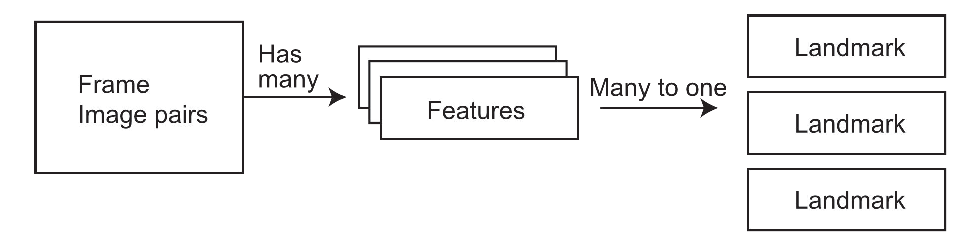
\includegraphics[width=1.0\linewidth]{designVO/frame-feature-landmark.pdf}
	\caption{基本数据结构及关系}
	\label{fig:frame-feature-landmark}
\end{figure}

好了,接下来我们要问,哪些算法负责提特征,哪些算法负责做三角化,又有哪些算法来处理优化问题呢?根据本书先前的介绍,我们认为SLAM由前后端组成。前端负责计算相邻图像的特征匹配,后端负责优化整个问题。在典型的实现中,二者应该有各自的线程。前端快速处理保证实时性,后端优化关键帧以保证良好的结果。所以整体来说,我们的程序有两个重要模块:

\begin{itemize}
\item 前端。我们往前端插入图像帧,前端负责提取图像中的特征,然后与上一帧进行光流追踪,通过光流结果计算该帧的定位。有必要时,应该补充新的特征点并做三角化。前端处理的结果将作为后端优化的初始值。
\item 后端。后端是一个较慢的线程,它拿到处理之后的关键帧和路标点,对它们进行优化,然后返回优化结果。后端应该控制优化问题的规模在一定范围内,不能随时间一直增长。
\end{itemize}

通过这样的分析,我们可以确定整个算法的框架,然后以喜闻乐见的流水线框图表达出来,如\autoref{fig:pipeline}。我们在前后端之间放了一个\textbf{地图}模块来处理它们之间的数据流动。由于前后端在分别的线程中处理数据,我们预想的流程应该是前端提取了关键帧后,往地图中添加新数据;后端检测到地图更新时,运行一次优化,然后再把地图中旧的关键帧和地图点去掉,保持优化的规模。

\begin{figure}[!htp]
    \centering
    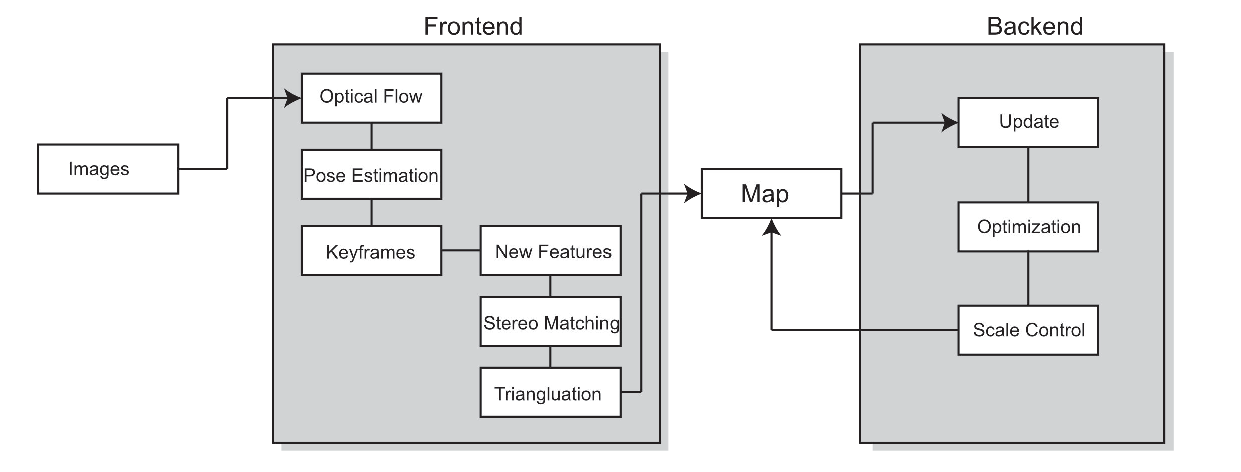
\includegraphics[width=1.0\linewidth]{designVO/pipeline.pdf}
    \caption{基本数据结构及关系}
    \label{fig:pipeline}
\end{figure}

这样我们就确定了大体上的系统流程,这有助于后续的编码实现。当然,除了核心算法之外,我们还需要一些周边的小模块来让系统更加方便,例如:

\begin{itemize}
\item 应该有一个相机类来管理相机的内外参和投影函数。
\item 我们需要一个配置文件管理类,方便从配置文件中读取内容。配置文件中可以记录一些重要参数方便我们作调整;
\item 因为最后算法在Kitti数据集上运行,所以我们需要按照Kitti的存储格式来读取图像数据,这也应该由一个单独的类来处理。
\item 我们需要一个可视化模块来观察系统的运行状态,否则就得对着一串串的数值挠头了。
\end{itemize}

这些模块虽然不算核心,但又不可或缺。限于篇幅,我们将周边代码交给读者自行阅读,在书中只介绍核心部分。

\section{实现}
\subsection{实现基础数据结构}
根据上一讲的讨论,我们先来实现帧、特征和路标点这三个类。对于基础数据结构,通常建议将它们设成struct,无需定义复杂的私有变量和接口。考虑到这些数据可能被多个线程访问和修改,在关键部分我们需要加上线程锁。

Frame结构设计如下:
\begin{lstlisting}[language=c++,caption=slambook2/ch13/include/myslam/frame.h]
struct Frame {
public:
    EIGEN_MAKE_ALIGNED_OPERATOR_NEW;
    typedef std::shared_ptr<Frame> Ptr;
    
    unsigned long id_ = 0;           // id of this frame
    unsigned long keyframe_id_ = 0;  // id of key frame
    bool is_keyframe_ = false;       // 是否为关键帧
    double time_stamp_;              // 时间戳,暂不使用
    SE3 pose_;                       // Tcw 形式Pose
    std::mutex pose_mutex_;          // Pose数据锁
    cv::Mat left_img_, right_img_;   // stereo images
    
    // extracted features in left image
    std::vector<std::shared_ptr<Feature>> features_left_;
    // corresponding features in right image, set to nullptr if no corresponding
    std::vector<std::shared_ptr<Feature>> features_right_;
    
public:  // data members
    Frame() {}
    
    Frame(long id, double time_stamp, const SE3 &pose, const Mat &left,
    const Mat &right);
    
    // set and get pose, thread safe
    SE3 Pose() {
        std::unique_lock<std::mutex> lck(pose_mutex_);
        return pose_;
    }
    
    void SetPose(const SE3 &pose) {
        std::unique_lock<std::mutex> lck(pose_mutex_);
        pose_ = pose;
    }
    
    /// 设置关键帧并分配并键帧id
    void SetKeyFrame();
    
    /// 工厂构建模式,分配id 
    static std::shared_ptr<Frame> CreateFrame();
};
\end{lstlisting}

我们定义Frame含有id、位姿、图像以及左右图像中的特征点。其中Pose会被前后端同时设置或访问,所以定义Pose的Set和Get函数,在函数内加锁。同时,Frame可以由静态函数构建,在静态函数中可以自动分配id。

然后是Feature:
\begin{lstlisting}[language=c++,caption=slambook2/ch13/include/myslam/feature.h]
struct Feature {
public:
    EIGEN_MAKE_ALIGNED_OPERATOR_NEW;
    typedef std::shared_ptr<Feature> Ptr;
    
    std::weak_ptr<Frame> frame_;         // 持有该feature的frame
    cv::KeyPoint position_;              // 2D提取位置
    std::weak_ptr<MapPoint> map_point_;  // 关联地图点
    
    bool is_outlier_ = false;       // 是否为异常点
    bool is_on_left_image_ = true;  // 标识是否提在左图,false为右图
    
public:
    Feature() {}
    
    Feature(std::shared_ptr<Frame> frame, const cv::KeyPoint &kp)
    : frame_(frame), position_(kp) {}
};
\end{lstlisting}

Feature最主要的信息是自身的2D位置,此外还有几个标志位描述它是否为异常点和是否提取在左相机中。我们可以通过一个Feature对象访问持有它的Frame以及它对应的路标。不过,Frame和MapPoint的实际持有权归地图所有,为了避免shared\_ptr产生的循环引用\footnote{简而言之,Frame持有了Feature的shared\_ptr,那么应避免Feature再持有Frame的shared\_ptr,否则两者相互引用,将导致智能指针无法自动析构。},这里使用了weak\_ptr。

最后是MapPoint,即路标点:
\begin{lstlisting}[language=c++,caption=slambook2/ch13/include/myslam/mappoint.h]
struct MapPoint {
public:
    EIGEN_MAKE_ALIGNED_OPERATOR_NEW;
    typedef std::shared_ptr<MapPoint> Ptr;
    unsigned long id_ = 0;  // ID
    bool is_outlier_ = false;
    Vec3 pos_ = Vec3::Zero();  // Position in world
    std::mutex data_mutex_;
    int observed_times_ = 0;  // being observed by feature matching algo.
    std::list<std::weak_ptr<Feature>> observations_;
    
    MapPoint() {}
    
    MapPoint(long id, Vec3 position);
    
    Vec3 Pos() {
        std::unique_lock<std::mutex> lck(data_mutex_);
        return pos_;
    }
    
    void SetPos(const Vec3 &pos) {
        std::unique_lock<std::mutex> lck(data_mutex_);
        pos_ = pos;
    };
    
    void AddObservation(std::shared_ptr<Feature> feature) {
        std::unique_lock<std::mutex> lck(data_mutex_);
        observations_.push_back(feature);
        observed_times_++;
    }
    
    void RemoveObservation(std::shared_ptr<Feature> feat);
    
    std::list<std::weak_ptr<Feature>> GetObs() {
        std::unique_lock<std::mutex> lck(data_mutex_);
        return observations_;
    }
    
    // factory function
    static MapPoint::Ptr CreateNewMappoint();
};
\end{lstlisting}

MapPoint最主要的是它的3D位置,即pos\_变量,同样需要对它上锁。它的observation\_变量记录了自己被哪些Feature观察到。因为Feature可能被判断为outlier,所以observation部分发生改动时也需要锁定。

至此我们就实现了基础的数据结构。在框架中,我们让地图类实际持有这些Frame和MapPoint的对象,所以还需要定义一个地图类:
\begin{lstlisting}[language=c++,caption=slambook2/ch13/include/myslam/map.h]
class Map {
public:
    EIGEN_MAKE_ALIGNED_OPERATOR_NEW;
    typedef std::shared_ptr<Map> Ptr;
    typedef std::unordered_map<unsigned long, MapPoint::Ptr> LandmarksType;
    typedef std::unordered_map<unsigned long, Frame::Ptr> KeyframesType;
    
    Map() {}
    
    /// 增加一个关键帧
    void InsertKeyFrame(Frame::Ptr frame);
    /// 增加一个地图顶点
    void InsertMapPoint(MapPoint::Ptr map_point);
    
    /// 获取所有地图点
    LandmarksType GetAllMapPoints() {
        std::unique_lock<std::mutex> lck(data_mutex_);
        return landmarks_;
    }
    /// 获取所有关键帧
    KeyframesType GetAllKeyFrames() {
        std::unique_lock<std::mutex> lck(data_mutex_);
        return keyframes_;
    }
    
    /// 获取激活地图点
    LandmarksType GetActiveMapPoints() {
        std::unique_lock<std::mutex> lck(data_mutex_);
        return active_landmarks_;
    }
    
    /// 获取激活关键帧
    KeyframesType GetActiveKeyFrames() {
        std::unique_lock<std::mutex> lck(data_mutex_);
        return active_keyframes_;
    }
    
    /// 清理map中观测数量为零的点
    void CleanMap();
    
private:
    // 将旧的关键帧置为不活跃状态
    void RemoveOldKeyframe();
    
    std::mutex data_mutex_;
    LandmarksType landmarks_;         // all landmarks
    LandmarksType active_landmarks_;  // active landmarks
    KeyframesType keyframes_;         // all key-frames
    KeyframesType active_keyframes_;  // all key-frames
    
    Frame::Ptr current_frame_ = nullptr;
    
    // settings
    int num_active_keyframes_ = 7;  // 激活的关键帧数量
};
\end{lstlisting}

地图以散列形式记录了所有的关键帧和对应的路标点,同时维护一个被激活的关键帧和地图点。这里\textbf{激活}的概念即我们所谓的\textbf{窗口},它会随着时间往前推动。后端将从地图中取出激活的关键帧、路标点进行优化,忽略其余的部分,达到控制优化规模的效果。当然,激活的策略是由我们自己定义的,简单的激活策略就是去除最旧的关键帧而保持时间上最新的若干个关键帧。在本书的实现中,我们只保留最新的7个关键帧。

\subsection{前端}
在定义了基础数据结构之后,我们来考虑前端的功能。前端需要根据双目图像确定该帧的位姿,不过实际实现的时候还存在一些不同的方法。例如,我们应该怎样使用右目的图像呢?是每一帧都和左右目各比一遍,还是仅比较左右目之一呢?在三角化的时候,我们是考虑左右目图像的三角化,还是考虑时间上前后帧的三角化呢?实际当中任意两张图像都可以做三角化(比如前一帧的左图对下一帧的右图),所以每个人实现起来也会不太一样。

为简单起见,我们先确定前端的处理逻辑:
\begin{enumerate}
\item 前端本身有\textbf{初始化}、\textbf{正常追踪}、\textbf{追踪丢失}三种状态。
\item 在初始化状态中,根据左右目之间的光流匹配,寻找可以三角化的地图点,成功时建立初始地图。
\item 追踪阶段中,前端计算上一帧的特征点到当前帧的光流,根据光流结果计算图像位姿。该计算只使用左目图像,不使用右目。
\item 如果追踪到的点较少,就判定当前帧为关键帧。对于关键帧,做以下几件事:
\begin{itemize}
\item 提取新的特征点;
\item 找到这些点在右图的对应点,用三角化建立新的路标点;
\item 将新的关键帧和路标点加入地图,并触发一次后端优化。
\end{itemize}
\item 如果追踪丢失,就重置前端系统,重新初始化。
\end{enumerate}

根据这个逻辑,前端处理流程大致如下:
\begin{lstlisting}[language=c++,caption=slambook2/ch13/src/frontend.cpp]
bool Frontend::AddFrame(myslam::Frame::Ptr frame) {
    current_frame_ = frame;
    switch (status_) {
        case FrontendStatus::INITING:
            StereoInit();
            break;
        case FrontendStatus::TRACKING_GOOD:
        case FrontendStatus::TRACKING_BAD:
            Track();
            break;
        case FrontendStatus::LOST:
            Reset();
            break;
    }
    
    last_frame_ = current_frame_;
    return true;
}
\end{lstlisting}

Track函数实现如下:
\begin{lstlisting}[language=c++,caption=slambook2/ch13/src/frontend.cpp]
bool Frontend::Track() {
    if (last_frame_) {
        current_frame_->SetPose(relative_motion_ * last_frame_->Pose());
    }
    
    int num_track_last = TrackLastFrame();
    tracking_inliers_ = EstimateCurrentPose();
    
    if (tracking_inliers_ > num_features_tracking_) {
        // tracking good
        status_ = FrontendStatus::TRACKING_GOOD;
    } else if (tracking_inliers_ > num_features_tracking_bad_) {
        // tracking bad
        status_ = FrontendStatus::TRACKING_BAD;
    } else {
        // lost
        status_ = FrontendStatus::LOST;
    }
    
    InsertKeyframe();
    relative_motion_ = current_frame_->Pose() * last_frame_->Pose().inverse();
    
    if (viewer_) viewer_->AddCurrentFrame(current_frame_);
    return true;
}
\end{lstlisting}
而在TrackLastFrame函数中,我们实际调用OpenCV的光流来追踪特征点:
\begin{lstlisting}[language=c++,caption=slambook2/ch13/src/frontend.cpp]
int Frontend::TrackLastFrame() {
    // use LK flow to estimate points in the right image
    std::vector<cv::Point2f> kps_last, kps_current;
    for (auto &kp : last_frame_->features_left_) {
        if (kp->map_point_.lock()) {
            // use project point
            auto mp = kp->map_point_.lock();
            auto px =
                camera_left_->world2pixel(mp->pos_, current_frame_->Pose());
                kps_last.push_back(kp->position_.pt);
            kps_current.push_back(cv::Point2f(px[0], px[1]));
        } else {
            kps_last.push_back(kp->position_.pt);
            kps_current.push_back(kp->position_.pt);
        }
    }
    
    std::vector<uchar> status;
    Mat error;
    cv::calcOpticalFlowPyrLK(
        last_frame_->left_img_, current_frame_->left_img_, kps_last,
        kps_current, status, error, cv::Size(21, 21), 3,
        cv::TermCriteria(cv::TermCriteria::COUNT + cv::TermCriteria::EPS, 30, 0.01),
        cv::OPTFLOW_USE_INITIAL_FLOW);
    
    int num_good_pts = 0;
    
    for (size_t i = 0; i < status.size(); ++i) {
        if (status[i]) {
            cv::KeyPoint kp(kps_current[i], 7);
            Feature::Ptr feature(new Feature(current_frame_, kp));
            feature->map_point_ = last_frame_->features_left_[i]->map_point_;
            current_frame_->features_left_.push_back(feature);
            num_good_pts++;
        }
    }
    
    LOG(INFO) << "Find " << num_good_pts << " in the last image.";
    return num_good_pts;
}
\end{lstlisting}

实现当中,我们尽量利用逻辑上的分拆,把复杂功能拆成一些短小的函数,直到底层函数才实际调用OpenCV或g2o来实现特定功能。这样有利用提升程序的可读性和复用性,比如初始化阶段的提特征和关键帧的提特征就可以使用同一个函数。我们建议读者自行阅读以节省篇幅(实际上前端一共不到400行代码)。

\subsection{后端}
相比前端,后端实现的逻辑会复杂一些。后端整体实现如下:
\begin{lstlisting}[language=c++,caption=slambook2/ch13/include/myslam/backend.h]
class Backend {
public:
    EIGEN_MAKE_ALIGNED_OPERATOR_NEW;
    typedef std::shared_ptr<Backend> Ptr;
    
    /// 构造函数中启动优化线程并挂起
    Backend();
    
    // 设置左右目的相机,用于获得内外参
    void SetCameras(Camera::Ptr left, Camera::Ptr right) {
        cam_left_ = left;
        cam_right_ = right;
    }
    
    /// 设置地图
    void SetMap(std::shared_ptr<Map> map) { map_ = map; }
    
    /// 触发地图更新,启动优化
    void UpdateMap();
    
    /// 关闭后端线程
    void Stop();
    
private:
    /// 后端线程
    void BackendLoop();
    
    /// 对给定关键帧和路标点进行优化
    void Optimize(Map::KeyframesType& keyframes, Map::LandmarksType& landmarks);
    
    std::shared_ptr<Map> map_;
    std::thread backend_thread_;
    std::mutex data_mutex_;
    
    std::condition_variable map_update_;
    std::atomic<bool> backend_running_;
    
    Camera::Ptr cam_left_ = nullptr, cam_right_ = nullptr;
};
\end{lstlisting}

后端在启动之后,将等待map\_update\_的条件变量。当地图更新被触发时,从地图中拿取激活的关键帧和地图点,执行优化:

\begin{lstlisting}[language=c++,caption=slambook2/ch13/src/backend.cpp]
void Backend::BackendLoop() {
    while (backend_running_.load()) {
        std::unique_lock<std::mutex> lock(data_mutex_);
        map_update_.wait(lock);
        
        /// 后端仅优化激活的Frames和Landmarks
        Map::KeyframesType active_kfs = map_->GetActiveKeyFrames();
        Map::LandmarksType active_landmarks = map_->GetActiveMapPoints();
        Optimize(active_kfs, active_landmarks);
    }
}
\end{lstlisting}

优化函数和我们之前使用的BA类似,只是数据要从Frame、MapPoint对象中获得:
\begin{lstlisting}[language=c++,caption=slambook2/ch13/src/backend.cpp]
void Backend::Optimize(Map::KeyframesType &keyframes,
    Map::LandmarksType &landmarks) {
    // setup g2o
    typedef g2o::BlockSolver_6_3 BlockSolverType;
    typedef g2o::LinearSolverCSparse<BlockSolverType::PoseMatrixType>
    LinearSolverType;
    auto solver = new g2o::OptimizationAlgorithmLevenberg(
    g2o::make_unique<BlockSolverType>(
    g2o::make_unique<LinearSolverType>()));
    g2o::SparseOptimizer optimizer;
    optimizer.setAlgorithm(solver);
    
    // pose 顶点,使用Keyframe id
    std::map<unsigned long, VertexPose *> vertices;
    unsigned long max_kf_id = 0;
    for (auto &keyframe : keyframes) {
        auto kf = keyframe.second;
        VertexPose *vertex_pose = new VertexPose();  // camera vertex_pose
        vertex_pose->setId(kf->keyframe_id_);
        vertex_pose->setEstimate(kf->Pose());
        optimizer.addVertex(vertex_pose);
        if (kf->keyframe_id_ > max_kf_id) {
            max_kf_id = kf->keyframe_id_;
        }
        
        vertices.insert({kf->keyframe_id_, vertex_pose});
    }
    
    // 路标顶点,使用路标id索引
    std::map<unsigned long, VertexXYZ *> vertices_landmarks;
    
    // K 和左右外参
    Mat33 K = cam_left_->K();
    SE3 left_ext = cam_left_->pose();
    SE3 right_ext = cam_right_->pose();
    
    // edges
    int index = 1;
    double chi2_th = 5.991;  // robust kernel 阈值
    std::map<EdgeProjection *, Feature::Ptr> edges_and_features;
    
    for (auto &landmark : landmarks) {
        if (landmark.second->is_outlier_) continue;
        unsigned long landmark_id = landmark.second->id_;
        auto observations = landmark.second->GetObs();
        for (auto &obs : observations) {
            if (obs.lock() == nullptr) continue;
            auto feat = obs.lock();
            if (feat->is_outlier_ || feat->frame_.lock() == nullptr) continue;
            
            auto frame = feat->frame_.lock();
            EdgeProjection *edge = nullptr;
            if (feat->is_on_left_image_) {
                edge = new EdgeProjection(K, left_ext);
            } else {
                edge = new EdgeProjection(K, right_ext);
            }
            
            // 如果landmark还没有被加入优化,则新加一个顶点
            if (vertices_landmarks.find(landmark_id) ==
            vertices_landmarks.end()) {
                VertexXYZ *v = new VertexXYZ;
                v->setEstimate(landmark.second->Pos());
                v->setId(landmark_id + max_kf_id + 1);
                v->setMarginalized(true);
                vertices_landmarks.insert({landmark_id, v});
                optimizer.addVertex(v);
            }
            
            edge->setId(index);
            edge->setVertex(0, vertices.at(frame->keyframe_id_));    // pose
            edge->setVertex(1, vertices_landmarks.at(landmark_id));  // landmark
            edge->setMeasurement(toVec2(feat->position_.pt));
            edge->setInformation(Mat22::Identity());
            auto rk = new g2o::RobustKernelHuber();
            rk->setDelta(chi2_th);
            edge->setRobustKernel(rk);
            edges_and_features.insert({edge, feat});
            
            optimizer.addEdge(edge);
            
            index++;
        }
    }
    
    // do optimization and eliminate the outliers
    optimizer.initializeOptimization();
    optimizer.optimize(10);
    
    int cnt_outlier = 0, cnt_inlier = 0;
    int iteration = 0;
    while (iteration < 5) {
        cnt_outlier = 0;
        cnt_inlier = 0;
        // determine if we want to adjust the outlier threshold
        for (auto &ef : edges_and_features) {
            if (ef.first->chi2() > chi2_th) {
                cnt_outlier++;
            } else {
                cnt_inlier++;
            }
        }
        double inlier_ratio = cnt_inlier / double(cnt_inlier + cnt_outlier);
        if (inlier_ratio > 0.5) {
            break;
        } else {
            chi2_th *= 2;
            iteration++;
        }
    }
    
    for (auto &ef : edges_and_features) {
        if (ef.first->chi2() > chi2_th) {
            ef.second->is_outlier_ = true;
            // remove the observation
            ef.second->map_point_.lock()->RemoveObservation(ef.second);
        } else {
            ef.second->is_outlier_ = false;
        }
    }
    
    LOG(INFO) << "Outlier/Inlier in optimization: " << cnt_outlier << "/"
    << cnt_inlier;
    
    // Set pose and lanrmark position
    for (auto &v : vertices) {
        keyframes.at(v.first)->SetPose(v.second->estimate());
    }
    for (auto &v : vertices_landmarks) {
        landmarks.at(v.first)->SetPos(v.second->estimate());
    }
}
\end{lstlisting}

后端相比前端更加简短一些,只有不到两百行,逻辑也十分简单。

\section{实验效果}
最后我们来看这个视觉里程计的实际运行效果。首先我们需要下载Kitti数据集:\url{http://www.cvlibs.net/datasets/kitti/eval_odometry.php}。它的odometry数据大约有22GB。下载之后解压得到若干个视频段,我们以第0段为例。编译本节程序之后,在配置文件config/default.yaml中填上数据对应的路径,在我的机器上为:
$$\text{dataset_dir: /media/xiang/Data/Dataset/Kitti/dataset/sequences/00}$$

然后,运行:
\begin{lstlisting}[language=sh,caption=终端输入:]
bin/run_kitti_stereo
\end{lstlisting}
之后即可看到定位输出,如\autoref{fig:snapshot-vo}所示。运行期间,程序将显示激活的关键帧和地图,它们应该随着镜头运动不断增长和消失。

\begin{figure}[!htp]
    \centering    
    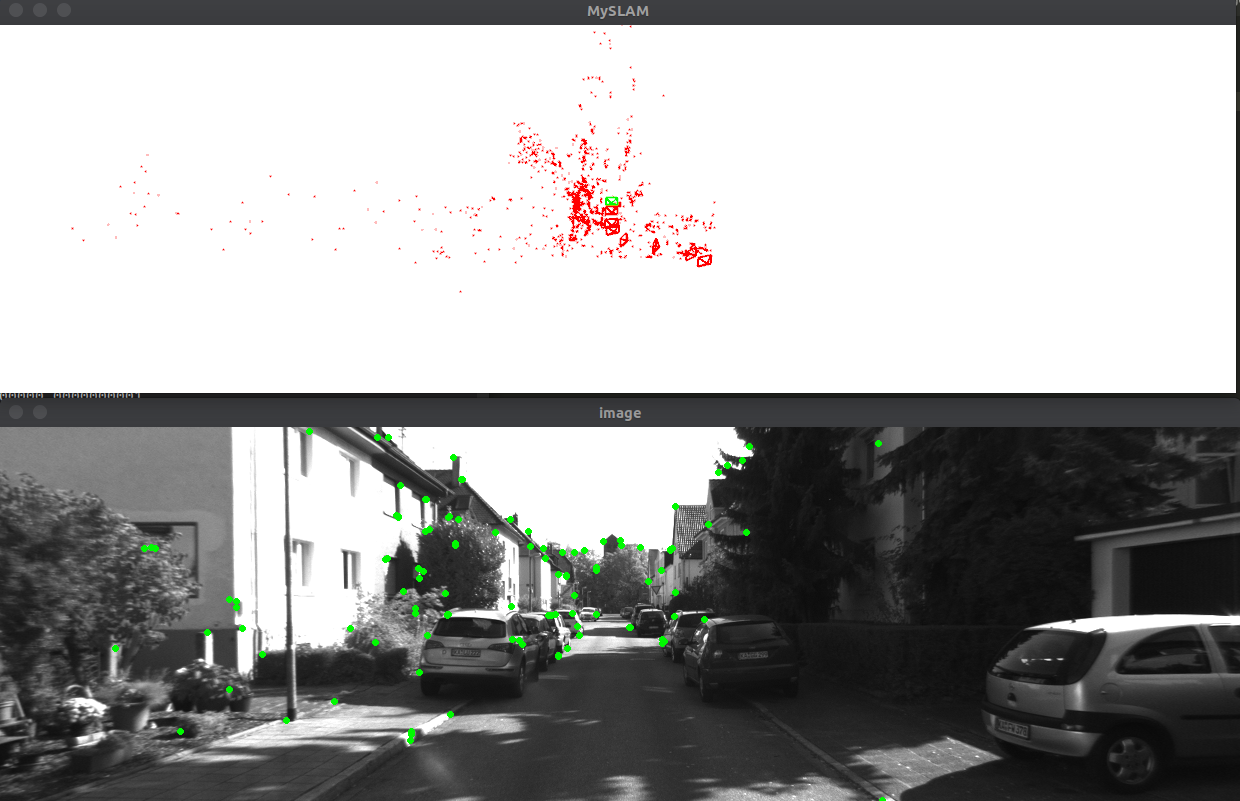
\includegraphics[width=0.9\linewidth]{designVO/snapshot-vo.png}\\
    \caption{视觉里程计运行截图}
    \label{fig:snapshot-vo}
\end{figure}

我们输出了该程序的单次运行耗时。在处理非关键帧时,我们的耗时约为16ms。处理关键帧时,由于新增了一步提特征点和寻找右图匹配,耗时会适当增多。并且,由于我们的地图目前会存储所有关键帧和地图点,在运行一段时间之后将导致内存增长。如果读者不需要全部地图,可以只保留激活的部分。

\section*{习题}
\begin{enumerate}
	\item 本书使用的C++技巧你都看懂了吗?如果有不明白的地方,使用搜索引擎补习相关的知识,包括:基于范围的for循环、智能指针、设计模式中的单例模式,等等。
	\item 考虑对本讲介绍的系统进行优化。例如,使用更快的提特征点方式(本节使用了GFTT,它并不算快),在左右匹配时使用1维的搜索而非二维的光流,使用直接法同时估计位姿与特征点对应关系,等等。
    \item* 为本节代码添加回环检测模块,在检测到回环时使用Pose Graph进行优化以消除累积误差。
\end{enumerate}
